\documentclass[french]{report}


\usepackage[T1]{fontenc}
%\usepackage[margin=1in]{geometry}
\usepackage[utf8]{inputenc}
\usepackage{lmodern}
\usepackage{babel}
\usepackage{pdfpages}

\usepackage{graphicx} 
\usepackage{amsmath,amssymb,amsthm}
%%%%% pour les graphics 
\usepackage{pgfplots}
\usepackage{tikz}
% pour le style
\usepackage{xcolor} % les couleurs du texte
\usepackage{ulem}
\usepackage{cancel}% pour supprimer du texte 

\usepackage[colorlinks=true, linkcolor=blue]{hyperref}
\usepackage{sectsty}

\usepackage{multicol}

\usepackage{inputenc}


\usepackage{listings}
\usepackage{color}
%%%%%% couleur des sections 
\sectionfont{\color{red}}
%\subsectionfont{\color{red}}


\lstset{
	language=SQL,
	keywordstyle=\color{blue},
	commentstyle=\color{green},
	stringstyle=\color{red},
	frame = single,
	breaklines= true,
	moredelim=[is][\color{yellow}]{}{()} % Colorer le nom de la fonction en jaune
}

%%%%%%%%%nouvelles commandes  
\addtolength{\oddsidemargin}{-.875in}
\addtolength{\evensidemargin}{-.875in}
\addtolength{\textwidth}{1.75in}
\addtolength{\topmargin}{-.875in}
\addtolength{\textheight}{1.75in}

\newcommand{\set}[1]{\left\lbrace#1\right\rbrace}
\newcommand{\sys}[1]{\left\lbrace\substack{#1}\right.}
\newcommand{\floor}[1]{\left\lfloor{#1}\right\rfloor}
\newcommand{\abs}[1]{\left|{#1}\right|}
\newcommand{\warning}{/!$\setminus$}




%%%%% defintions des couleurs 
\definecolor{skyblue}{RGB}{135, 206, 235}
\definecolor{darkgreen}{RGB}{0, 150, 0}

\definecolor{myblue}{rgb}{0, 0.13, 0.60}
\definecolor{mygrey}{gray}{0.85}
\definecolor{lblue}{rgb}{0.22,0.45,0.70}


\title{Rapport Base de données}
\author{Augustin Fourmy - Elazar Cohen}

\begin{document}
	\maketitle
	\tableofcontents
	\newpage
	
	\chapter{Rendu 1}
	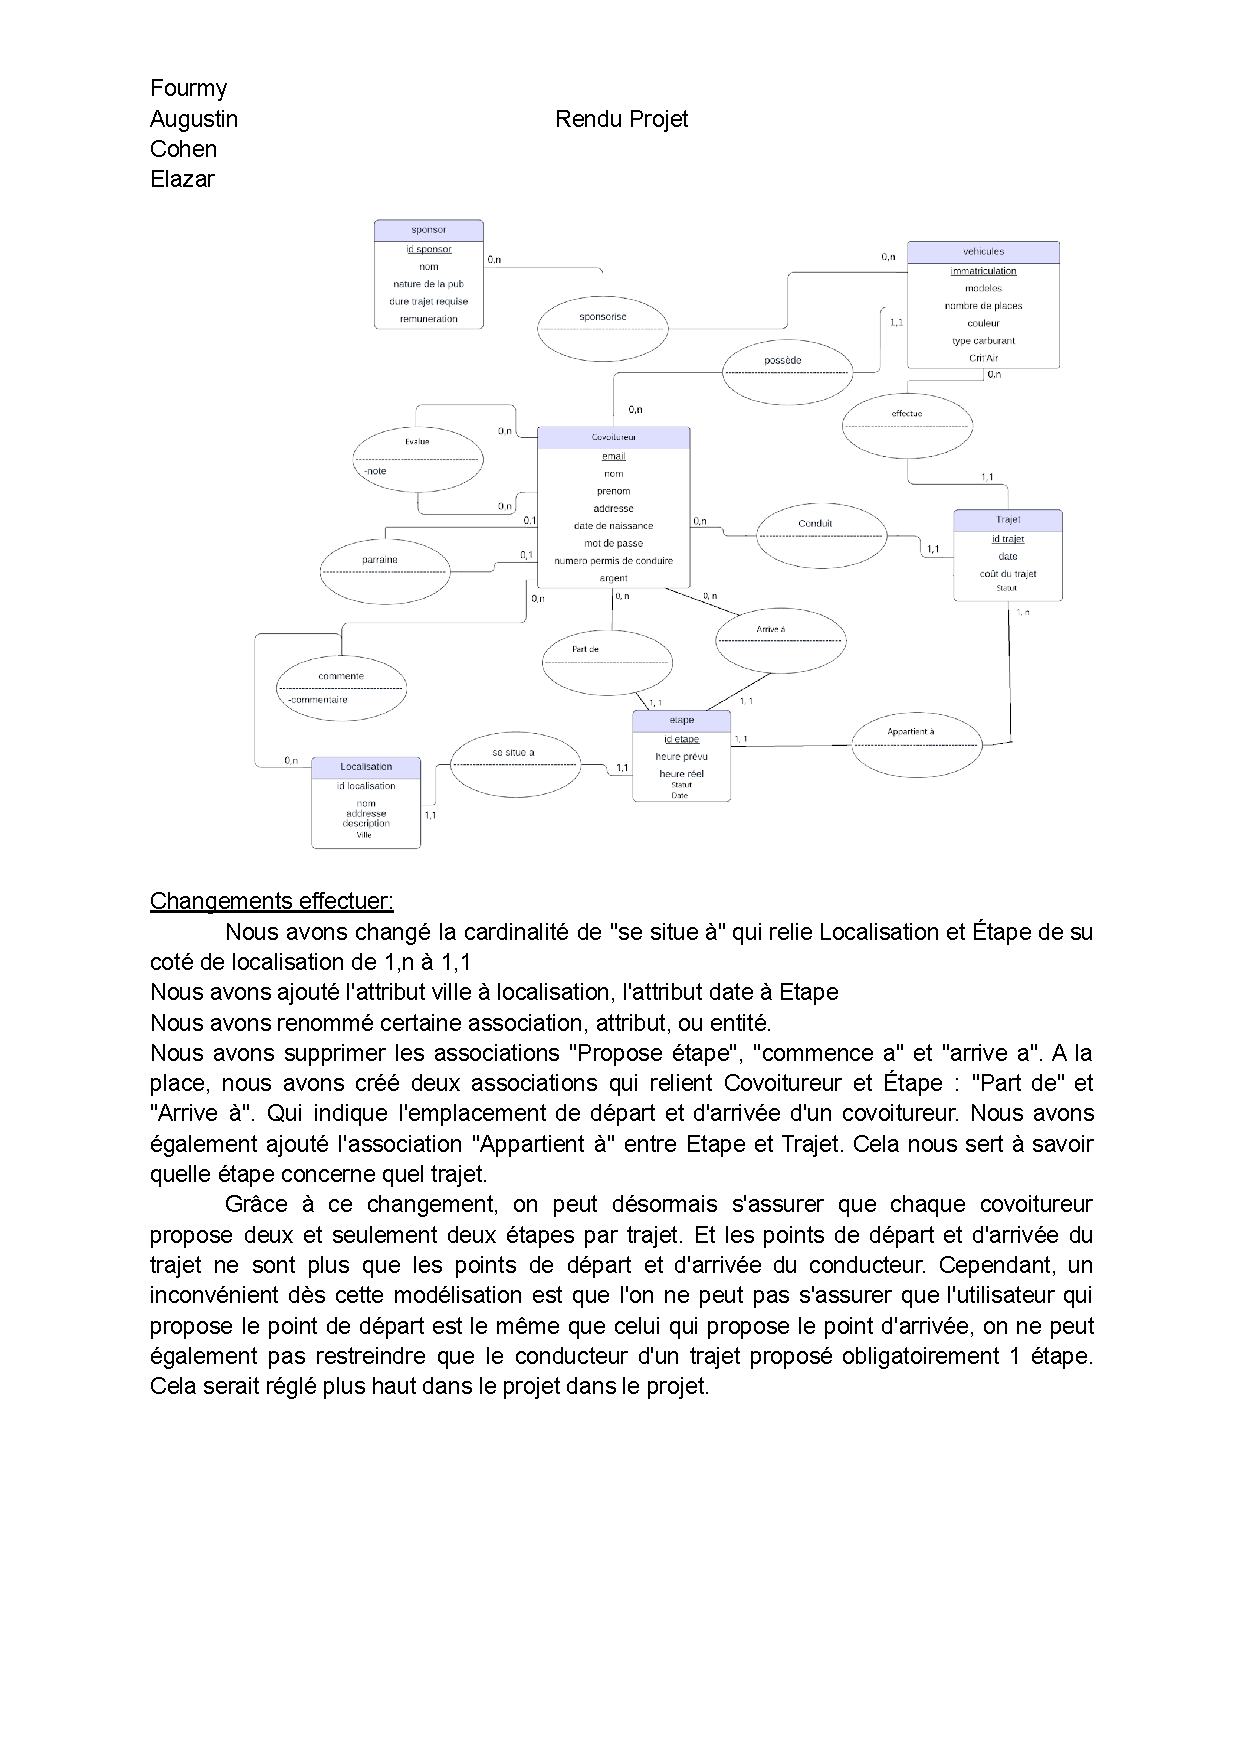
\includepdf[pages=-]{rendu1.pdf}
	
	\chapter{Rendu 2}
	




\section{Traduction du Schéma Entité-Association}
	En traduisant le schéma entité-association on obtient les tables suivantes:
	\begin{itemize}
		\item Covoitureur(\underline{email}, nom, prenom, addresse, date\_de\_naissance, mdp, num\_permis, argent, parrain)
		\item Localisation(\underline{id\_localisation}, nom, adresse, description, ville)
		\item Etape(\underline{id\_etape}, heure\_prevue, heure\_reel, statut, date, trajet, est\_depart\_de, est\_arriver\_de, localisation)
		\item Trajet(\underline{id\_trajet}, date, cout, statut, vehicule, conducteur, nb\_km, duree)
		\item Vehicules(\underline{immatriculation}, modele, nb\_place, couleur, carburant, crit\_air, proprietaire)
		\item Sponsor(\underline{id\_sponsor}, nom, nature, duree\_requise, remmuneration)
		
		
		\item Sponsorise(\underline{id\_sponsor, immatriculation})
		\item Commente(\underline{email, id\_localisation}, commentaire)
		\item Evalue(\underline{source, cible}, note)
	\end{itemize}
	On a les clefs étrangères:
	\begin{itemize}
		\item Sponsorise(id\_sponsor) fais reférence à Sponsor(id\_sponsor)
		\item Sponsorise(immatriculation) fais reférence à Vehicules(immatriculation)
		\item Commente(email) fais reférence à Covoitureur(email)
		\item Commente(id\_localisation) fais reférence à Localisation(id\_localisation)
		\item Evalue(source) fais reférence à Covoitureur(email)
		\item Evalue(cible) fais reférence à Covoitureur(email)
		\item Covoitureur(parrain) fais reférence à Covoitureur(email)
		\item Vehicule(proprietaire) fais référence à Covoitureur(email)
		\item Trajet(vehicule) fais référence à Vehicules(immatriculation)
		\item Trajet(conducteur) fais référence à Covoitureur(email)
		\item Etape(trajet) fais référence  à Trajet(id\_trajet)
		\item Etape(est\_depart\_de) fais référence à Covoitureur(email)
		\item Etape(est\_arriver\_de) fais référence à Covoitureur(email)
		\item Etape(localisation) fais référence à Localisation(id\_localisation)
	\end{itemize}
	
	\section{Implémentation}	
	\subsection{Schéma de la base et Justification des choix}
	\begin{center}
		\begin{tabular}{|c|c|c|}
			\hline
			\multicolumn{3}{|c|}{Covoitureur}\\
			\hline
			Nom & Type & Contrainte \\
			\hline
			email & varchar(100) & PRIMARY KEY \\\hline
			nom & varchar(50) & NOT NULL \\\hline
			prenom & varchar(50) & NOT NULL \\\hline
			addresse & varchar(100) & NOT NULL \\\hline
			date\_de\_naissance & date & NOT NULL \\\hline
			mdp & char(64) & NOT NULL \\\hline
			num\_permis & char(12) & \\\hline
			argent & numeric(11, 2) & default 0 \\\hline
			parrain & varchar(100)	& REFERENCES Covoitureur(email) ON DELETE SET NULL \\\hline
			\multicolumn{3}{|c|}{CHECK (email  $< >$ parrain)}\\\hline
		\end{tabular}
		
		\begin{tabular}{|c|c|c|}
			\hline
			\multicolumn{3}{|c|}{Localisation}\\
			\hline
			Nom & Type & Contrainte \\
			\hline
			id\_localisation & serial & PRIMARY KEY \\\hline
			nom & varchar(50) & NOT NULL \\\hline
			addresse & varchar(100) & NOT NULL \\\hline
			description & varchar(500) & \\\hline
			ville & varchar(64) & NOT NULL \\\hline
		\end{tabular}
		\begin{tabular}{|c|c|c|}
			\hline
			\multicolumn{3}{|c|}{Etape}\\
			\hline
			Nom & Type & Contrainte \\
			\hline
			id\_etape & serial & PRIMARY KEY \\\hline
			heure\_prevue & time & NOT NULL \\\hline
			heure\_reel & time &  \\\hline
			status & bool & default false \\\hline
			date & date & NOT NULL \\\hline
			trajet & int & NOT NULL REFERENCES trajet(id\_trajet) ON DELETE CASCADE \\\hline
			est\_depart\_de & varchar(100) & REFERENCES Covoitureur(email) ON DELETE CASCADE \\\hline
			est\_arriver\_de & varchar(100) & REFERENCES Covoitureur(email) ON DELETE CASCADE \\\hline
			localisation & int & NOT NULL REFERENCES Localisation(id\_localisation) ON DELETE CASCADE\\\hline
			\multicolumn{3}{|c|}{CHECK((est\_depart\_de IS NULL AND est\_arriver\_de IS NOT NULL)} \\
			\multicolumn{3}{|c|}{OR (est\_depart\_de IS NOT NULL AND est\_arriver\_de IS NULL))}\\\hline
		\end{tabular}
		
		
		
		\begin{tabular}{|c|c|c|}
			\hline
			\multicolumn{3}{|c|}{Vehicules}\\
			\hline
			Nom & Type & Contrainte \\
			\hline
			immatriculation & char(7) & PRIMARY KEY \\\hline
			modele & varchar(55) & NOT NULL \\\hline
			nb\_places & int & NOT NULL \\\hline
			couleur & varchar(60) & NOT NULL \\\hline
			carburant & varchar(50) & NOT NULL \\\hline
			crit\_air & char(1) & NOT NULL CHECK(crit\_air IN ('E', '1', '2', '3', '4', '5')) \\\hline
			proprietaire & varchar(100) & NOT NULL REFERENCES Covoirureur(email) \\
			&&  ON DELETE CASCADE ON UPDATE CASCADE \\\hline
		\end{tabular}
		
		\begin{tabular}{|c|c|c|}
				\hline
			\multicolumn{3}{|c|}{Trajet}\\
			\hline
			Nom & Type & Contrainte \\
			\hline
			id\_trajet & serial & PRIMARY KEY \\\hline
			date & date & NOT NULL \\\hline
			cout & numeric(9, 2) & NOT NULL \\\hline
			statut & bool & default false \\\hline
			vehicule & char(7) & NOT NULL REFERENCES Vehicules(immatriculation) ON DELETE CASCADE \\\hline
			localisation & int & NOT NULL REFERENCES Localisation(id\_localisation) ON DELETE CASCADE \\\hline
			nb\_km & int & CHECK(nb\_km $>$= 0)  \\\hline
			duree & interval &\\\hline
		\end{tabular}
		
		\begin{tabular}{|c|c|c|}
			\hline
			\multicolumn{3}{|c|}{Sponsor}\\
			\hline
			Nom & Type & Contrainte \\
			\hline
			id\_sponsor & serial & PRIMARY KEY \\\hline
			nom & varchar(75) & NOT NULL \\\hline
			nature & varchar(500) & NOT NULL \\\hline
			duree\_requise & interval & NOT NULL \\\hline
			remuneration & numeric(11, 2) & NOT NULL\\\hline
		\end{tabular}
		
		\begin{tabular}{|c|c|c|}
			\hline
			\multicolumn{3}{|c|}{Sponsorise}\\
			\hline
			Nom & Type & Contrainte \\
			\hline
			id\_sponsor & int & REFERENCES Sponsor(id\_sponsor)\\\hline
			immatriculation & char(7) & REFERENCES Vehicules(immatriculation) \\\hline
			\multicolumn{3}{|c|}{PRIMARY KEY (id\_sponsor, immatriculation)}\\\hline
		\end{tabular}
		
		\begin{tabular}{|c|c|c|}
			\hline
			\multicolumn{3}{|c|}{Commente}\\
			\hline
			Nom & Type & Contrainte \\
			\hline
			email & varchar(100) & REFERENCES Covoitureur(email) \\
			& & ON DELETE CASCADE ON UPDATE CASCADE \\\hline
			id\_localisation & int & REFERENCES Localisation(id\_localisation) \\\hline
			commentaire & varchar(500) & NOT NULL \\\hline
			\multicolumn{3}{|c|}{PRIMARY KEY (email, id\_localisation)}\\\hline
		\end{tabular}
		
		\begin{tabular}{|c|c|c|}
			\hline
			\multicolumn{3}{|c|}{Evalue}\\
			\hline
			Nom & Type & Contrainte \\
			\hline
			source & varchar(100) & REFERENCES Covoitureur(email)  \\
			& & ON DELETE CASCADE ON UPDATE CASCADE\\\hline
			cible & varchar(100) & REFERENCES Covoitureur(email)  \\
			& & ON DELETE CASCADE ON UPDATE CASCADE\\\hline
			note & int & NOT NULL \\\hline
			\multicolumn{3}{|c|}{PRIMARY KEY (source, cible)}\\\hline
			\multicolumn{3}{|c|}{CHECK (source  $< >$ cible)}\\\hline
		\end{tabular}
	\end{center}
	Nous avons fais certain choix sur les types:
	\begin{itemize}
		\item Les mot de passent sont stocker comme des chaines de caractères d'exactement 64 caractères car ils seront hacher avant que leur forme hexadécimal soit stocker.
		\item  Nous séparons la date et les heures pour ne pas permettre de renseigné le décalage de deux jours
		\item Nous avons rajouter un attribut longueur pour pouvoir réaliser les demandes supplémentaires
	\end{itemize}

	\subsection{Contraintes non Garantie}
	Il y a des contraintes que nous n'avons pas pus implémentés dans le schéma:
	\begin{itemize}
		\item Il nous est impossible de vérifier que l'e-mail de l'utilisateur est valide
		\item Il en est de même pour les plaques d'immatriculations 
		\item  Nous ne pouvons pas nous assurer que les covoitureurs  déposent exactement deux étape pour un trajet
	\end{itemize}
	\pagebreak
	\section{Demande supplémentaire}
	Nous avons créer des vues pour répondre aux contraintes supplémentaire qui nous ont été demander
	\begin{itemize}
		\item Obtenir les 10 premiers points de rendez-vous les plus f
		\begin{lstlisting}[language=SQL]
CREATE VIEW TopLocation AS (
	SELECT adresse, ville, COUNT(id_etape) FROM etape
	NATURAL JOIN Localisation
	GROUPE BY adresse, ville
	ORDER BY COUNT(id_etape) DESC
	LIMIT 10
);
		\end{lstlisting}
		\item Le nombre de kilomètre parcourus pour chaque sponsor
		\begin{lstlisting}[language=SQL]
CREATE VIEW SponsorKm AS (
	SELECT id_sponsor, nom, SUM(nb_km) FROM Sponsor
	NATURAL JOIN Sponsorise NATURAL JOIN Vehicules
	JOIN Trajet ON vehicules = immatriculation
	GROUP BY id_sponsor, nom
);
		\end{lstlisting}
	\end{itemize}
	

 
	
	\chapter{Rendu 3}
	\section{Ajout par rapport au deuxième rapport}
	\subsection{Dans le dump}
		\begin{enumerate}
			\item 
				dans la table covoitureur nous avions mis la taille des mot de passe a 64 or pour hacher le mot de passe la taille du mot de passe est de 60. 
			\item 
				Dans la table trajet nous avons rajouter un durée trajet de type interval et nb\_km de type numeric(6,3) car en avons beosin pour les VIEW demander 
			\item 	
				dans la table trajet, nous avons enlevé une relation redondante qui étais l'association conduit car nous pouvons y accéder avec un \textit{JOIN} entre le trajet et les véhicules dans le shema entité association.
			\item 
				nous avons enlever la date dans étape, en effet c'est la même information que la date dans trajet, elle est donc inutile.
		\end{enumerate}
	\subsection{Génération du dump}
		Dans le rapport 2 nous avions générer quelque données avec une IA. Mais cette fois nous avons créer un fichier python qui permet de générer un dump aléatoire avec autant de données que souhaité. vous pourrez trouver le fichier pour générer ce dump dans un dossier Dumpmaker et il faut lancer le fichier dumpmaker.py. (la génération des covoitureurs avec le hashage des mot de passe est un peu long)
		

\section{Explication du site}
	\subsection{Menu}
		\begin{itemize}
			\item 
				Si vous n'êtes pas connecte vous avez accès que a l'accueil, a connexion et les statistiques. 
			\item 
				Si vous êtes connecte en revanche vous pourrez apercevoir l'accueil, votre profil, les trajets, les trajets en cours, se déconnecter et les statistiques . 
		\end{itemize}
		
	\subsection{Accueil}
		en arrivant sur le site vous pourrez trouver une belle page d'accueil ou vous pourrez a votre guise regarder les trajets existants. 
		vous trouverez aussi un menu avec une page de connexion et les statistiques du site. 
	\subsection{Connexion}
		vous pouvez maintenant vous connecter avec votre compte si vous en avez un, ou dans le cas contraire vous inscrire en rentrant votre email, nom,prénom,etc. 
		une fois inscris vous pouvez vous connecter a votre compte qui vous dirige vers l'accueil. Vous avez maintenant accès a l'ensemble du menu pour naviguer dans le site.
	
	\subsection{Profil} 
		Comme dit plus haut si vous êtes connecte vous pouvez allez sur votre profil. 
		Le profil est divisé en 4 parties:
		\begin{enumerate}
			\item
				Les données de l'utilisateur: elles permettent de voir les données comme le nom, le prénom,l'argent,si on a le permis pouvoir l'enlever ou le rajouter si il nous a été retirer par les policiers ou le FBI. On peut aussi voir son parrain si on en a un et les filleuls.
			\item 
				La deuxième parti est pour voir les véhicules en sélectionnant la plaque d'immatriculation et on peut aussi ajouter un véhicule.  
				Des qu'on voit un véhicule :
				\begin{itemize}
					 \item 
					 	on peut voir les données de son véhicule avec le nombre de place ou encore la couleur 
					 \item 
					 	on peut aussi modifier son véhicule en modifiant la plaque ou la couleur, etc .
					 \item  
					 	la troisième parti du véhicules est pour sponsoriser son véhicule en choisissant le sponsor parmi les différents sponsor 
				\end{itemize}
			\item 
				la troisième parti parti du profil est la liste des différents trajet déjà effectué.

				\begin{table}[h!]
					\centering
					\begin{tabular}{cc}
						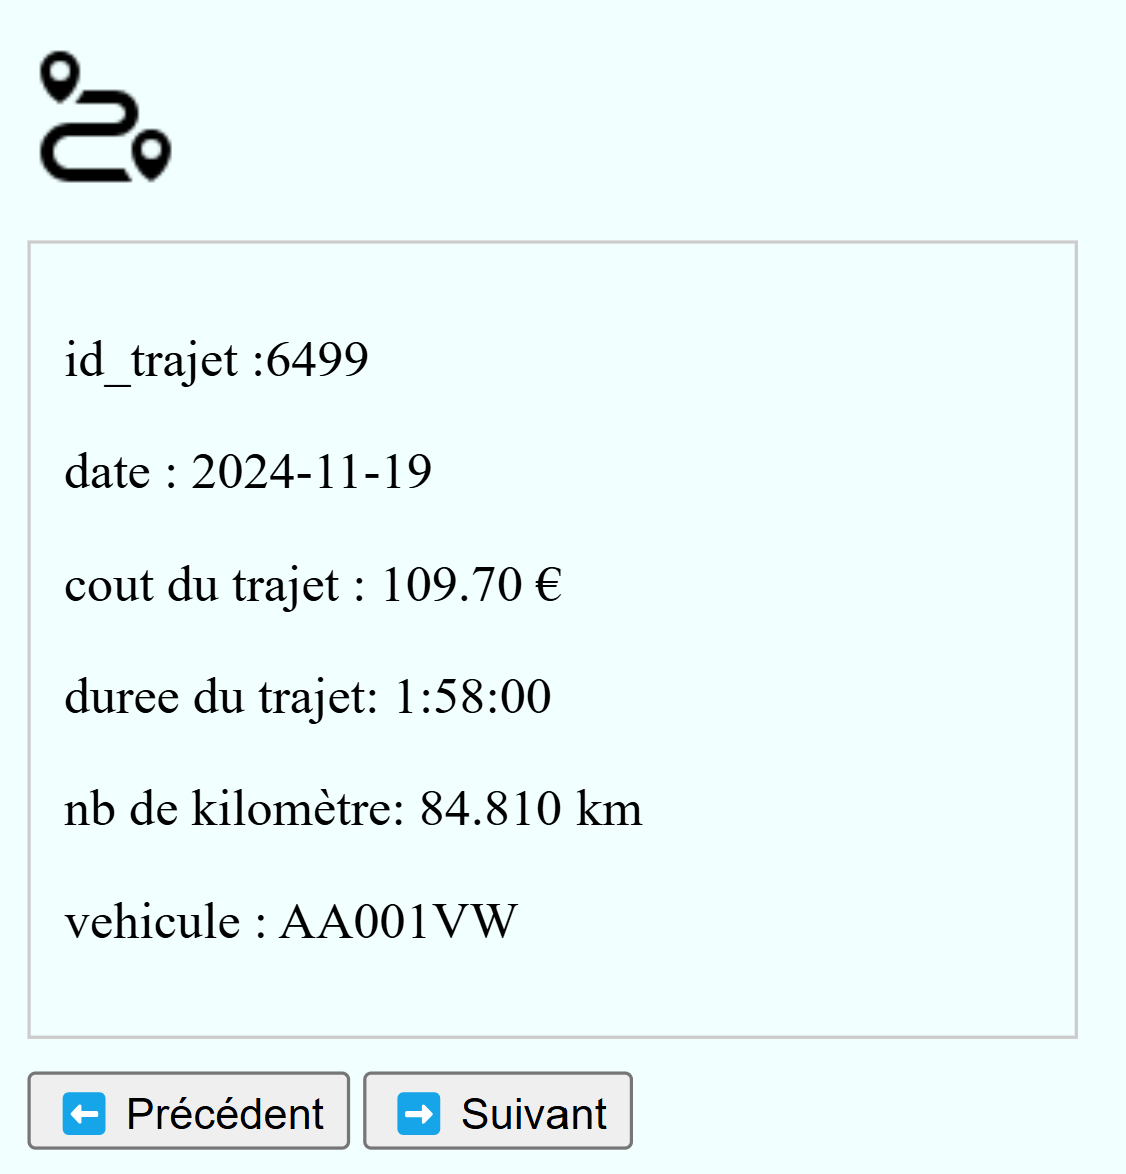
\includegraphics[width=0.4\textwidth]{trajet.png} & 
						\begin{minipage}[c]{0.5\textwidth}
							Comme vous pouvez le voir sur l'image, j'ai utilisé un peu de JavaScript pour pouvoir naviguer parmi les trajets passés.
						\end{minipage}
					\end{tabular}
					\caption{Navigation avec JavaScript}
					\label{fig:exemple}
				\end{table}
			\item 
				la dernière parti c'est les opérations sur votre compte en raison des couts des trajets ou si vous avez conduit certains trajets vous recevez de l'argent. 	
		\end{enumerate}
	\subsection{Trajet}		
		Sur le menu il y'a une page de trajet, elle permet de proposer un nouveau trajet avec une étape et d'arrivée.
		on peut aussi tout les trajets avec les information nécessaire ou si on veut en savoir plus on peux cliquer sur plus d'information pour voir précisément le trajet et pouvoir rajouter une étape au trajet.On peut aussi noter le conducteur ou encore allez dans plus d'info sur l'étape et écrire un commentaire de la localisation. \\
		Si un utilisateur propose une nouvelle étape le covoitureur depuis son compte peut voir l'étape qui a été proposé, l'accepter a sa guise et finalisée le trajet. Il peut aussi le réouvrir pour permettre a un utilisateur de proposer une nouvelle étape.\\
		un covoitureur (caractérisé par son permis de conduire) peut créer un nouveau trajet en renseignant une etape de départ et d'arriver avec le cout du trajet, le nombre de kilomètre que fais le trajet le temps espéré etc.
		
		 
	
	\subsection{Trajet en cours}
		La page trajet en cours permet a l'utilisateur de voir ses trajets et de pouvoir trier pour voir seulement les trajets en cours ou les trajets passées, etc.
	
	\subsection{Déconnexion}
		ce n'est pas une page mais on peut se déconnecter ce qui permet de supprimer de la session l'utilisateur et le redirige vers l'accueil sans toutes les options.
	
	\subsection{Statistiques}
		les statistiques permettent de voir les lieux les 10 lieux les plus visités du site et le nombre de km parcourus au total et avec des voitures sponsorisés 
		
\section{Explication du code}
nous allons expliquer quelques bout de code important 
	\subsection{La clé secrète}
		Pour générer la clé sécrète nous avons utilisé le module secrets de python.
		\begin{lstlisting}[language=python]
			secrets.token_urlsafe(100)
		\end{lstlisting}
		Ce qui nous a permis de générer une clé secrète de 100 caractères. 
	\subsection{L'accueil}	
		nous avons écris une route supplémentaire pour arriver directement sur l'accueil au lancement du site
		\begin{lstlisting}[language=python]
			@app.route("/")
			def main()->None:
			return redirect(url_for("accueil"))
		\end{lstlisting}
	
	\subsection{Éviter de réécrire la base de la template}
		pour éviter de réécrire dans chaque template la base du html nous avons créer une page $base.html$ qui nous sert de base a toute les templates. 
		\begin{lstlisting}[language=html]
			<!DOCTYPE html>
			<html lang="en">
			<head>
			<meta charset="UTF-8">
			<meta name="viewport" content="width=device-width, initial-scale=1.0">
			<link rel="stylesheet" type="text/css" href="../static/base.css">
			  
			<title>  </title>
			</head>
			<header>
			<nav>
			<ul>
			<li><a href="/accueil">Accueil</a></li>
			
			<li><a href="/connexion">Connexion</a></li>
			
			<li><a href="/statistiques">Statistique</a></li>
			
			
			</ul>  
			</nav>
			</header>
			<body>
			<div id = "content">
			 
			
			</div>
			</body>
			</html>
		\end{lstlisting}
		
		En faisant ca cela nous permet d'avoir une template sans avoir a réécrire toute la base html et surtout si nous voulons modifier le menu ou le css du menu nous avons pas besoin de le modifier dans toute les pages. Nous avons juste a écrire comme ci dessous. 
		\pagebreak
		\begin{lstlisting}[language=html]
			
			 <link rel="stylesheet" type="text/css" href="../static/connexion.css"> 
			            
			<li><a href="/connexion">Connexion</a></li>
			
			
			
			
		\end{lstlisting} 
		
	\subsection{Petits icons}
		Dans le profil nous avons ajouté des petits icons pour rendre le visuel plus sympathique. 
	
	\section{Quelques requêtes SQL intéressante}
		Nous avons fait pas mal de requêtes SQL dans ce projet notamment pour afficher des données ou des trajets et/ou faire des update de la base de donnée pour ajouter un véhicule ou le modifier ou encore proposer une étape et créer un trajet. Voici quelques requêtes SQL.
		\begin{lstlisting}[language=SQL]
SELECT id_trajet, date, cout_trajet, nom, prenom, nombre_places 
FROM trajet AS t 
JOIN vehicules AS v ON t.vehicule = v.immatriculation 
JOIN covoitureur AS c ON c.email = v.proprietaire
WHERE date >= '%s-%s-%s'
ORDER BY date LIMIT 20 OFFSET %s;
		\end{lstlisting}
		
		\begin{lstlisting}[language=SQL]
SELECT trajet.id_trajet,trajet.date,cout_trajet FROM etape
JOIN trajet ON etape.id_trajet = trajet.id_trajet 
JOIN vehicules ON trajet.vehicule = vehicules.immatriculation 
	JOIN covoitureur ON covoitureur.email = vehicules.proprietaire
WHERE est_depart_de = %s AND est_depart_de <> email  AND trajet.date <= %s  AND trajet.status = True ORDER BY trajet.date;

		\end{lstlisting}
		passager avec covoitureur la personne connecté
	
\section{Organisation du travail}
	Nous nous sommes repartis les taches équitablement.En effet Elazar s'est occupé de la connexion l'inscription et le profil et Augustin s'est occupé des trajets , trajets en cours et les statistiques.
		

		
		
		
		
		
		
		
		
		
		
		
		
		
		
		
		
		
		
		
		
		
		
		
		
		
	
	

	
	
	
	
	
	
	
	
	
	
	
	
	
	
	
	
	
	
	
	
	
	
	
	
	

	
\end{document}
